\documentclass{beamer}

\mode<presentation> {
  \usetheme{Warsaw}
  \setbeamercovered{transparent}
}

\usepackage{ucs}
\usepackage[utf8x]{inputenc}
\usepackage[czech]{babel}
\usepackage{palatino}
\usepackage{graphicx}
\usepackage{fancyvrb}
\usepackage{minted}

\begin{document}
\setbeamertemplate{caption}{\insertcaption}

\title{Validace konfiguračních souborů Flow123d}
\author[Bc. Tomáš Křížek]{{\large Bc. Tomáš Křížek}\\{\scriptsize Vedoucí práce: Jiří Vraný, Ph.D.}}
\institute[TUL]{Technická univerzita v Liberci}
\date{4.~června~2015}

\begin{frame}
	\titlepage
\end{frame}

\begin{frame}
	\frametitle{Úvod do problematiky}
	\begin{block}{Flow123d}
		\begin{itemize}
			\item simulace transportu látek
			\item jedním ze vstupů jsou \textbf{konfigurační soubory} s parametry simulace
		\end{itemize}
	\end{block}

	\begin{block}{GeoMop}
		\begin{itemize}
			\item nástroj pro usnadnění práce uživatelům Flow123d
			\item jedna součást je grafický editor konfiguračních souborů
		\end{itemize}
	\end{block}
\end{frame}

\begin{frame}
	\frametitle{Proces validace konfiguračních souborů}
	\begin{figure}[h]
		\centering
		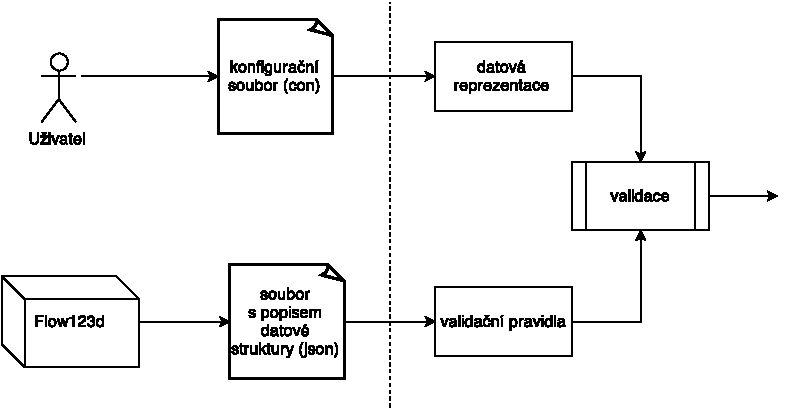
\includegraphics[width=\linewidth]{con_validation.pdf}
	\end{figure}
\end{frame}

\begin{frame}
	\frametitle{Konfigurační soubory Flow123d}
	\begin{itemize}
		\item pro inicializaci tříd v C++
		\item formát CON
		\item psány ručně -- možnost zanesení chyb $\rightarrow$ nutnost \textbf{validace}
		\item datová struktura
			\begin{itemize}
				\item tvoří strom -- vnořené záznamy a pole; listy -- skalární hodnoty
				\item je \textit{proměnná} (závislá na konkrétní verzi Flow123d)
				\item podporuje \textit{reference}
				\item umožňuje zkrácený zápis některých záznamů nebo polí (\textit{autokonverze})
			\end{itemize}
	\end{itemize}
\end{frame}

% \begin{frame}
% 	\frametitle{Základní datové typy}
% 	\begin{columns}[c]
% 		\begin{column}{0.35\textwidth}
% 			$\bullet$ skalární hodnoty
% 		\end{column}
% 		\begin{column}{0.65\textwidth}
% 			\texttt{3, 5.2, "string", \dots}
% 		\end{column}
% 	\end{columns}
% 	\vspace{5mm}
% 	\begin{columns}[c]
% 		\begin{column}{0.35\textwidth}
% 			$\bullet$ pole (homogenní)
% 		\end{column}
% 		\begin{column}{0.65\textwidth}
% 			\texttt{[1.0, 0.0, \dots]}
% 		\end{column}
% 	\end{columns}
% 	\vspace{5mm}
% 	\begin{columns}[c]
% 		\begin{column}{0.35\textwidth}
% 			$\bullet$ záznamy
% 		\end{column}
% 		\begin{column}{0.65\textwidth}
% 	       \texttt{\{} \\
% 	        \texttt{~~\textit{file} = "dual\_por.pvd",} \\
% 	        \texttt{~~\textit{format} = \{\dots\},} \\
% 	        \texttt{~~\textit{name} = "flow\_output\_stream"} \\
% 	      \texttt{\}}
% 		\end{column}
% 	\end{columns}
% 	% \vspace{5mm}
% 	% \begin{columns}[c]
% 	% 	\begin{column}{0.35\textwidth}
% 	% 		$\bullet$ abstraktní záznamy
% 	% 	\end{column}
% 	% 	\begin{column}{0.65\textwidth}
% 	%        \texttt{\{} \\
% 	%         \texttt{~~\textit{TYPE} = "vtk",} \\
% 	%         \texttt{~~\dots} \\
% 	%       \texttt{\}}
% 	% 	\end{column}
% 	% \end{columns}
% \end{frame}

% \begin{frame}[fragile]
% 	\frametitle{Soubor s popisem datové struktury}
% 	$\bullet$ sada pravidel popsaná pomocí JSON \\
% 	$\bullet$ odlišná pro různé verze Flow123d \\
% 	$\bullet$ Příklad: \\
% 	\begin{columns}[c]
% 		\begin{column}{0.05\textwidth}
% 		\end{column}
% 		\begin{column}{0.35\textwidth}
% 			pole, které obsahuje \\jeden až dva prvky \\
% 			\vspace{1.6cm}
% 			prvky jsou reálná čísla větší rovna nule
% 		\end{column}
% 		\begin{column}{0.6\textwidth}
% 			\footnotesize\begin{minted}{json}
% 			[
% 			  {
% 			    "id" : "57a7a5e1a86f94ad",
% 			    "input_type" : "Array",
% 			    "range" : [1, 2],
% 			    "subtype" : "6b1c4ede475775aa"
% 			  },
% 			  {
% 			    "id" : "6b1c4ede475775aa",
% 			    "input_type" : "Double",
% 			    "name" : "Double",
% 			    "full_name" : "Double",
% 			    "range" : [0, 1.79769e+308]
% 			  }
% 			]
% 			\end{minted}
% 		\end{column}
% 	\end{columns}
% \end{frame}

\begin{frame}[fragile]
	\frametitle{Ukázka použití}
	\begin{itemize}
		\item v budoucnu součástí interaktivního grafického editoru
		\item aktuálně rozhraní pro konzoli pro účely demonstrace a testování
	\end{itemize}
	\noindent
	\footnotesize\begin{Verbatim}[commandchars=\\\{\}]
		\textcolor{blue}{$} python3 cli.py demo/example.con -f demo/1.8.2.json
		\textcolor{green}{VALID}
	\end{Verbatim}
	\footnotesize\begin{Verbatim}[commandchars=\\\{\}]
		\textcolor{blue}{$} python3 cli.py demo/invalid.con -f demo/1.8.2.json
		\textcolor{red}{INVALID}
		\textit{/problem/primary_equation/solver}: Invalid TYPE 'PSsc' 
		    for LinSys
		\textit{/problem/secondary_equation/balance/cumulative}: Expecting 
		    type Bool
	\end{Verbatim}
	\normalsize
\end{frame}

\begin{frame}
	\frametitle{Výsledky práce}
	Vytvořené rozhraní pro validaci umožňuje
	\begin{itemize}
		\item načíst konfigurační soubor ve formátu CON,
		\item z tohoto souboru vytvořit datovou reprezentaci s ohledem na
		speciální vlasnosti formátu (reference, autokonverze),
		\item načíst soubor s popisem očekávané struktury souboru a dynamicky mu přizpůsobit proces validace,
		\item určit zda je soubor validní pro danou verzi Flow123d a případně identifikovat nalezené nesrovnalosti.
	\end{itemize}
	Budoucí využití:
	\begin{itemize}
		\item určení verze konfiguračního souboru a převod mezi verzemi,
		\item generování nápovědy a dokumentace
	\end{itemize}
\end{frame}

% \begin{frame}
% 	\frametitle{Budoucí využití}
% 	\begin{itemize}
% 		\item vytvořené rozhraní bude využito v aplikaci GeoMop
% 		\item validace bude probíhat interaktivně v grafickém editoru
% 		\item proces validace umožňí:
% 			\begin{itemize}
% 				\item určit správnost zadaných dat
% 				\item určit verzi načteného konfiguračního souboru
% 			\end{itemize}
% 		\item datová struktura byla navržena tak, aby umožnila:
% 			\begin{itemize}
% 				\item generování nápovědy v rámci aplikaci,
% 				\item generování dokumentace
% 			\end{itemize}
% 	\end{itemize}
% \end{frame}

\begin{frame}{}{}
\begin{center}
\huge Děkuji za pozornost.
\end{center}
\end{frame}

\end{document}